% Gemini theme
% https://github.com/anishathalye/gemini
%
% We try to keep this Overleaf template in sync with the canonical source on
% GitHub, but it's recommended that you obtain the template directly from
% GitHub to ensure that you are using the latest version.

\documentclass[final]{beamer}

% ====================
% Packages
% ====================

\usepackage[T1]{fontenc}
\usepackage{lmodern}
\usepackage[size=custom,width=120,height=72,scale=1.0]{beamerposter}
\usetheme{gemini}
\usecolortheme{gemini}
\usepackage{graphicx}
\usepackage{booktabs}
\usepackage{tikz}
\usepackage{pgfplots}
\usepackage{caption}

% ====================
% Lengths
% ====================

% If you have N columns, choose \sepwidth and \colwidth such that
% (N+1)*\sepwidth + N*\colwidth = \paperwidth
\newlength{\sepwidth}
\newlength{\colwidth}
%\setlength{\sepwidth}{0.015\paperwidth}
%\setlength{\colwidth}{0.225\paperwidth}
\setlength{\sepwidth}{0.025\paperwidth}
\setlength{\colwidth}{0.30\paperwidth}
\setlength{\paperwidth}{46.8in} % A0 width: 46.8in
\setlength{\paperheight}{33.1in} % A0 height: 33.1in

\newcommand{\separatorcolumn}{\begin{column}{\sepwidth}\end{column}}

% ====================
% Chuck's addition per: https://tex.stackexchange.com/a/426090
% ====================

\pgfplotsset{compat=1.16}
\makeatletter
\let\@@magyar@captionfix\relax
\makeatother

% ====================
% Title
% ====================

\title{Axon AI's Solution to the 2nd YouTube-8M Video Understanding Challenge}

%\author{Alyssa P. Hacker \inst{1} \and Ben Bitdiddle \inst{2} \and Lem E. Tweakit \inst{2}}
\author{Choongyeun Cho, Benjamin Antin, Sanchit Arora, Shwan Ashrafi, Peilin Duan, Dang The Huynh, Lee James, Hang Tuan Nguyen, Mojtaba Solgi, Cuong Van Than}

% \institute[shortinst]{\inst{1} Some Institute \samelineand \inst{2} Another Institute}
\institute{Axon AI}

% ====================
% Body
% ====================

\begin{document}

\begin{frame}[t]
\begin{columns}[t]
\separatorcolumn

\begin{column}{\colwidth}

  \begin{block}{PRE-PROCESS}
    \textbf{Observation}: videos associated with a same label form a cluster, whereas others are separated to some degree.
	\begin{figure}
    	\centering
    	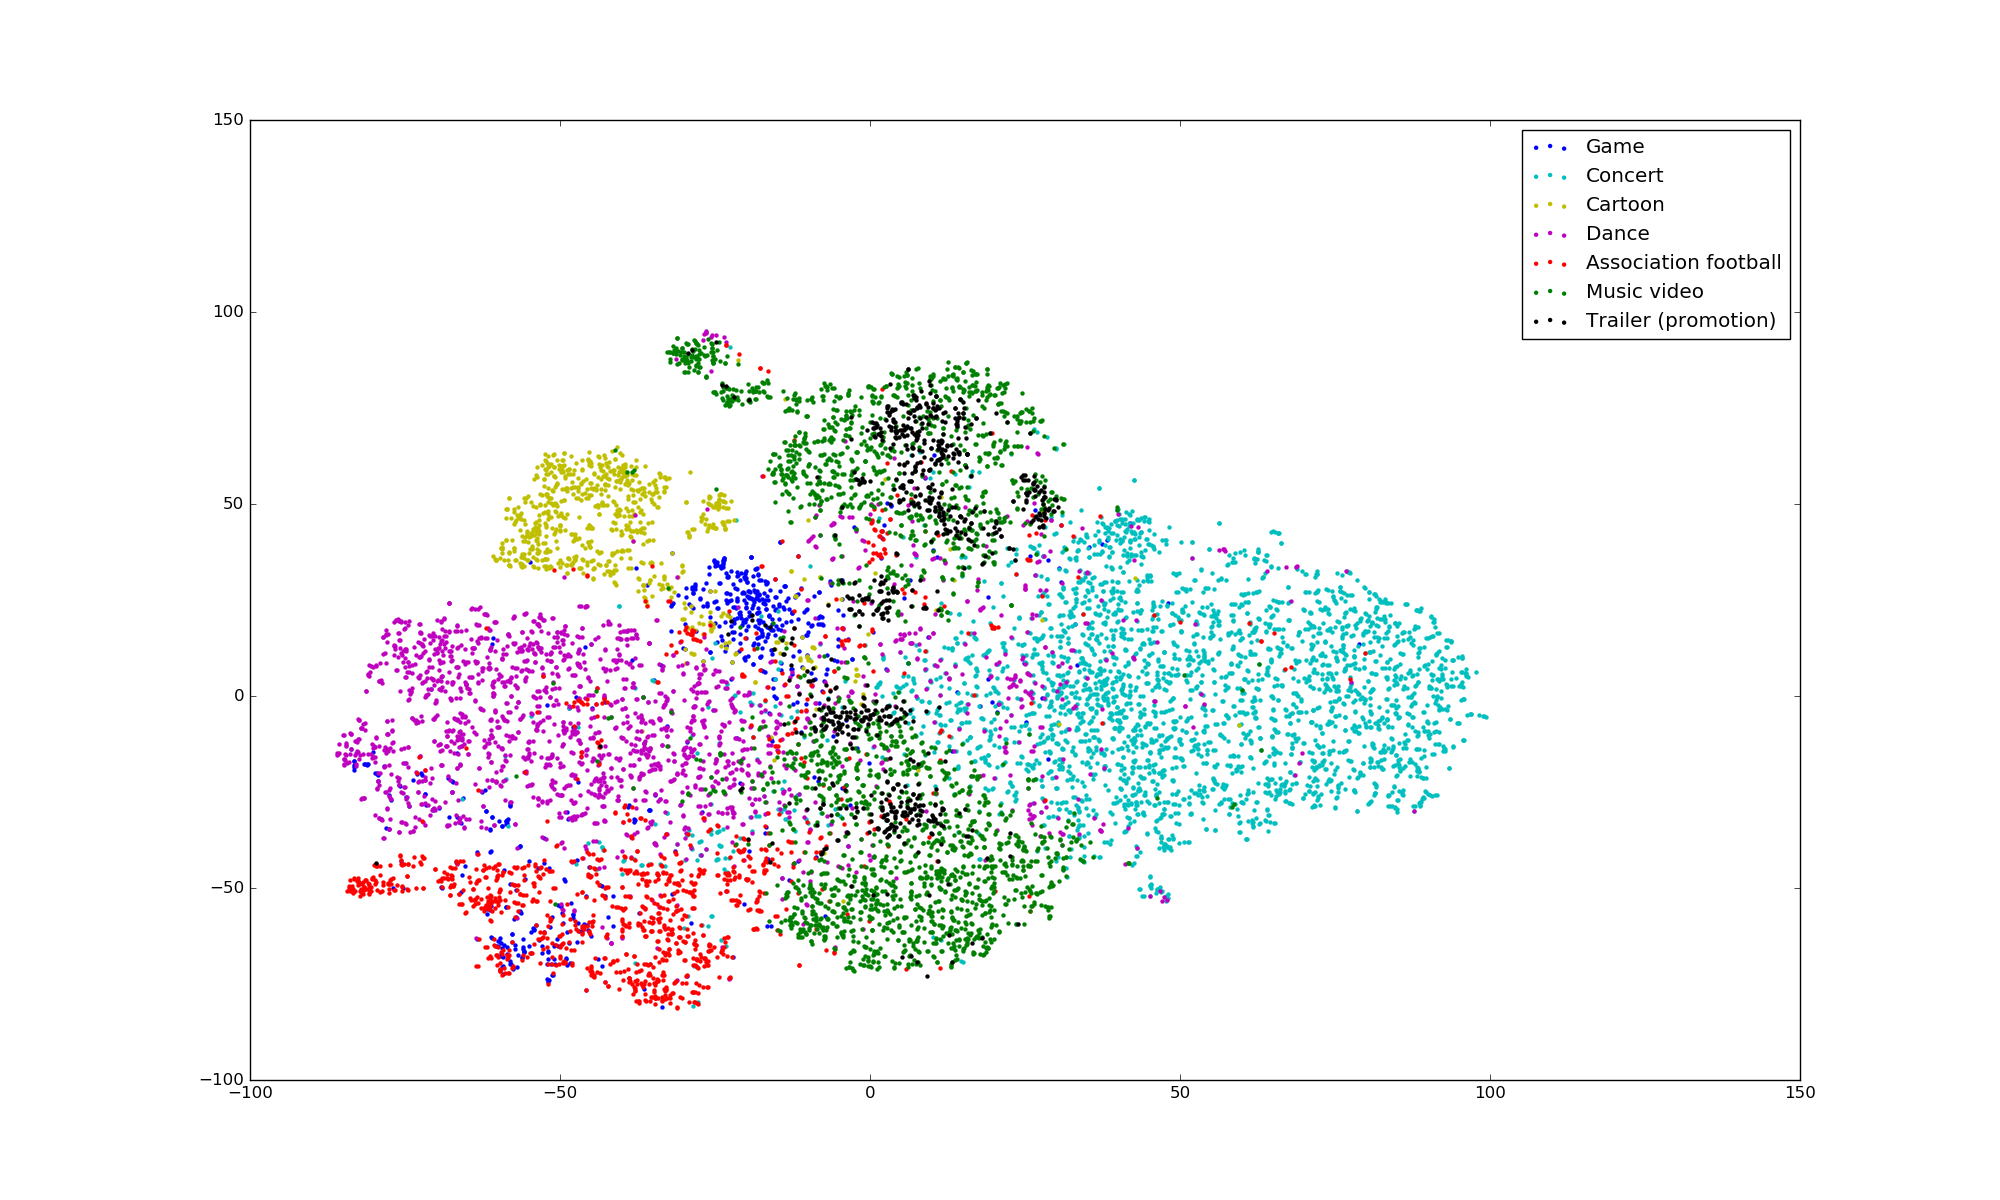
\includegraphics[width=1.0\linewidth]{../figures/tsne-vfeat-large2.png}
		\caption{TSNE plot of visual features for a few selected classes}	
    \end{figure}
  \end{block}
  
  \begin{alertblock}{Data augmentation}
    Data augmentation is for visual features only, by adding small noise to the feature vector.
	\begin{equation}
		x'_i = x_i + \gamma Z, Z \sim \mathcal{N}(0, \sigma^2)
	\end{equation}
    
    \textbf{Over-sampling:} a single label with less than $10^4$ samples. For each sample $x_i$, find $K$ nearest neighbors $x_j$ (L2-distance)
    \begin{itemize}
      \item Interpolation
      \begin{equation}
          x'_i = x_i + \lambda_i (x_j - x_i)
      \end{equation}
      \item Extrapolation
      \begin{equation}
          x'_i = x_i + \lambda_e (x_i - x_j)
      \end{equation}
    \end{itemize}
    \textbf{Sub-sampling} (random-sampling): a single label with more than $10^4$ samples.
  \end{alertblock}
  	\begin{figure}
    	\centering
    	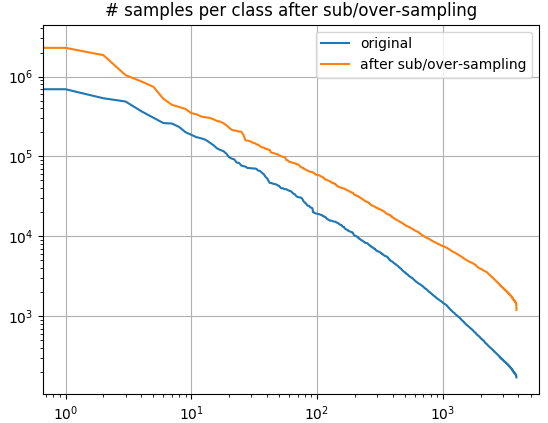
\includegraphics[width=0.6\linewidth]{../figures/new_num_samples_per_class_cropped.png}
		\caption{Label counts before and after data augmentation in feature space.Before data augmentation: 5,001,275; After data augmentation: \textbf{23,590,464} (472\%)
}	
    \end{figure}
\end{column}

\separatorcolumn

% ====================
% Column 2
% ====================

\begin{column}{\colwidth}
  \begin{block}{TRAINING}
    Identify powerful and efficient baseline models regardless of their model sizes:
  \begin{itemize}
    \item Training set: train????.tfrecord + validate???[0-4,6-9].tfrecord
    \item Validation set: validate???5.tfrecord
    \item All models are kept original, trained with Adam optimizer (LR = 0.0002 with exponential decay 0.8 for every 4M samples)
    \item Context gating version: y = $\sigma (W \cdot x + b) \circ x$
  \end{itemize}

	    \begin{table}[h!]
  \begin{center}
    \begin{tabular}{ c | c }
    \toprule
      \textbf{Model family} & \textbf{Brief description of individual models}  \\
    %\hline
    %\hline
    \midrule
            LP & Gated NetVLAD with 256 clusters \\
    \hline
            LP & Gated NetFV with 128 clusters \\
    \hline
            BoW & Gated soft-DBoW with 4096 clusters \\
    \hline
            BoW & Soft-DBoW with 8000 clusters \\
    \hline
            LP &  Gated NetRVLAD with 256 clusters \\
    \hline
            RNN & Gated recurrent unit (GRU) \\
            & with 2 layers and 1024 cells per layer \\
    \hline
            RNN & LSTM with 2 layers and 1024 cells per layer \\
    \bottomrule
    \end{tabular}
    \caption{A set of 7 single baseline models before ensembling}
    \label{tab:single_models}
  \end{center}
\end{table}

	\begin{table}[h!]
  \begin{center}
    \begin{tabular}{l|c} % <-- Alignments: 1st column left, 2nd middle and 3rd right, with vertical lines in between
    \toprule
            \textbf{Experiment} & \textbf{Test GAP (\%)} \\
      %\hline
      %\hline
   	\midrule
            Single baseline model (gated NetVLAD) & 85.75 (Val GAP) \\
      \hline
            Single gated NetVLAD model + video-level MoE model\\
            trained with augmented dataset in feature space & 85.98 (Val GAP) \\
      \hline
            Single gated NetVLAD model + regularized DNN\\
            exploiting label relationship & 87.88 (Val GAP) \\
      \hline
      A simple average ensembling of all of the 7 models & 88.27 \\
      \hline
      A simple average ensembling of two sets of\\ all of the 7 models (14 models in total) & 88.62  \\
      \hline
            Ensembled using learned weights &  \textbf{88.73} \\
      \hline
            Distilled model & \textbf{87.29} \\
      \bottomrule
    \end{tabular}
    \caption{GAP performance per experiment}
    \label{tab:gap}
  \end{center}
\end{table}
  \end{block}
  
  	\begin{alertblock}{Submodels ensembling}
    \begin{itemize}
    	\item Simple average.
        \item \textbf{Per-model linearly-weighted average.}
		\item Per-model and per-class linearly-weighted average.
    \end{itemize}
    
\begin{table}[h!]
  	\begin{center}
    \begin{tabular}{ l | c }
    \toprule
    \textbf{Single baseline model} & \textbf{Per-model weight} \\
    %\hline
    %\hline
    \midrule
            Gated NetVLAD & 0.2367 \\
    \hline
            Gated NetFV & 0.1508 \\
    \hline
            Gated soft-DBoW & 0.1590 \\
    \hline
            Soft-DBoW & 0.1000 \\
    \hline
            Gated NetRVLAD & 0.1968\\
    \hline
            GRU & 0.1306 \\
    \hline
            LSTM & 0.0621 \\
    \bottomrule
    \end{tabular}
    \caption{Learned weights for 7 baseline models}
    \label{tab:learned_weights}
  	\end{center}
\end{table}
    
    \end{alertblock}

\end{column}

\separatorcolumn

% ====================
% Column 3
% ====================

\begin{column}{\colwidth}

  \begin{block}{POST-PROCESS}

    Exploit correlation and diversity of \textbf{video label relationship}, by using an extra regularization term.
\begin{equation}
\min_{\boldsymbol{W}, \Omega}\sum_{i=1}^{N}l(f(x_i),y_i) +\frac{\lambda_{1}}{2}\sum_{l=1}^{L-1}||\boldsymbol{W}_l||_F^2 + \lambda_{2}\cdot \textnormal{tr}(\boldsymbol{W}_{L-1}\Omega^{-1}\boldsymbol{W}_{L-1}^{T}) 
\end{equation}
$\textnormal{s.t. } \Omega\succeq0$.
The optimal $\Omega \in \mathbb{R}^{C \times C}$ can be derived as:
\begin{equation}
\Omega = \frac{(\boldsymbol{W}_{L-1}^T \boldsymbol{W}_{L-1})^\frac{1}{2}}{\textnormal{tr}((\boldsymbol{W}_{L-1}^T \boldsymbol{W}_{L-1})^\frac{1}{2})}
\end{equation}



  \end{block}

  \begin{block}{MODEL COMPRESSION}

    Approach: training a student model ( < 1GB) based on a teacher model (ensemble of 7 baseline models).
    \begin{itemize}
		\item Student model: \textbf{NetVLAD} with the last FC of 800 hidden weights (instead of 1024)
        \item Loss function: weighted sum of two cross-entropy losses (with teacher model prediction $\tilde{p}$ and with ground truth $q$)
        \begin{equation}
        	L=\lambda\cdot CE(p,\overset{\sim}{p}) + (1-\lambda)\cdot CE(p,q)
        \end{equation}
    \end{itemize}
  \end{block}
  
    \begin{alertblock}{Knowledge distillation}
      \begin{table}[h!]
      \begin{center}
        \begin{tabular}{ l | c }
        \toprule
          \textbf{Experiment} & \textbf{Test GAP}  \\
        \midrule
                Ensembled using learned weights & 88.73 \\
        \hline
                Distilled model & 87.29 \\
        \bottomrule
        \end{tabular}
        \caption{GAP performance after knowledge distillation}
        \label{tab:distillation}
      \end{center}
    \end{table}
  \end{alertblock}

  \begin{block}{References}

    \nocite{*}
    \footnotesize{\bibliographystyle{plain}\bibliography{axonai-eccv2018-poster}}

  \end{block}

\end{column}

\separatorcolumn

% ====================
% Column 4
% ====================


\separatorcolumn


\end{columns}
\end{frame}

\end{document}
